\section{在线贝叶斯 CIR 适配}

\subsection{共享物理状态与 Frozen 对照}

Frozen 与 Bayes 使用同一 checkpoint、同一 acquisition CIR 先验、同一 \texttt{dd\_soft} tail 规则与同一接收波形；两臂的神经权重都冻结。Frozen 在整个会话中保持 acquisition CIR 不变；Bayes 只把 CIR 的均值与协方差按合法观测递推。因而两臂的差异被限制在物理状态后验上，BER 差可以归因于 CIR 适配，而不是网络容量、Pilot 预算或训练数据。

\texttt{dd\_soft} tail 指：用当前帧最后 \texttt{max\_delay} 个 Data 位置的模型软判决 $\tanh(z_t/2)$ 递推下一帧的信道尾部，与离线课程训练中的 \texttt{online\_soft} 规则对齐，尺度 $\alpha=1.0$。该规则只读接收波形与模型输出，不读 Data 标签。共享 tail 规则是公平比较的关键。若 Frozen 使用与离线训练不一致的 tail 递推，或 Bayes 额外获得更长的历史，两臂的差异就会混入 tail 协议而不是 CIR 后验。本文在确认前固定 \texttt{dd\_soft}、$\alpha=1.0$ 与历史长度，使两臂只在 CIR 是否更新上不同；tail 复用与独立前向的逐位一致性也在成本 profile 中单独核对。图 3 给出在线闭环：物理状态条件化冻结网络，网络输出软判决，软判决与 Adapt Pilot 共同进入贝叶斯更新，更新后的状态只用于下一帧。

\begin{figure}[htbp]
\centering
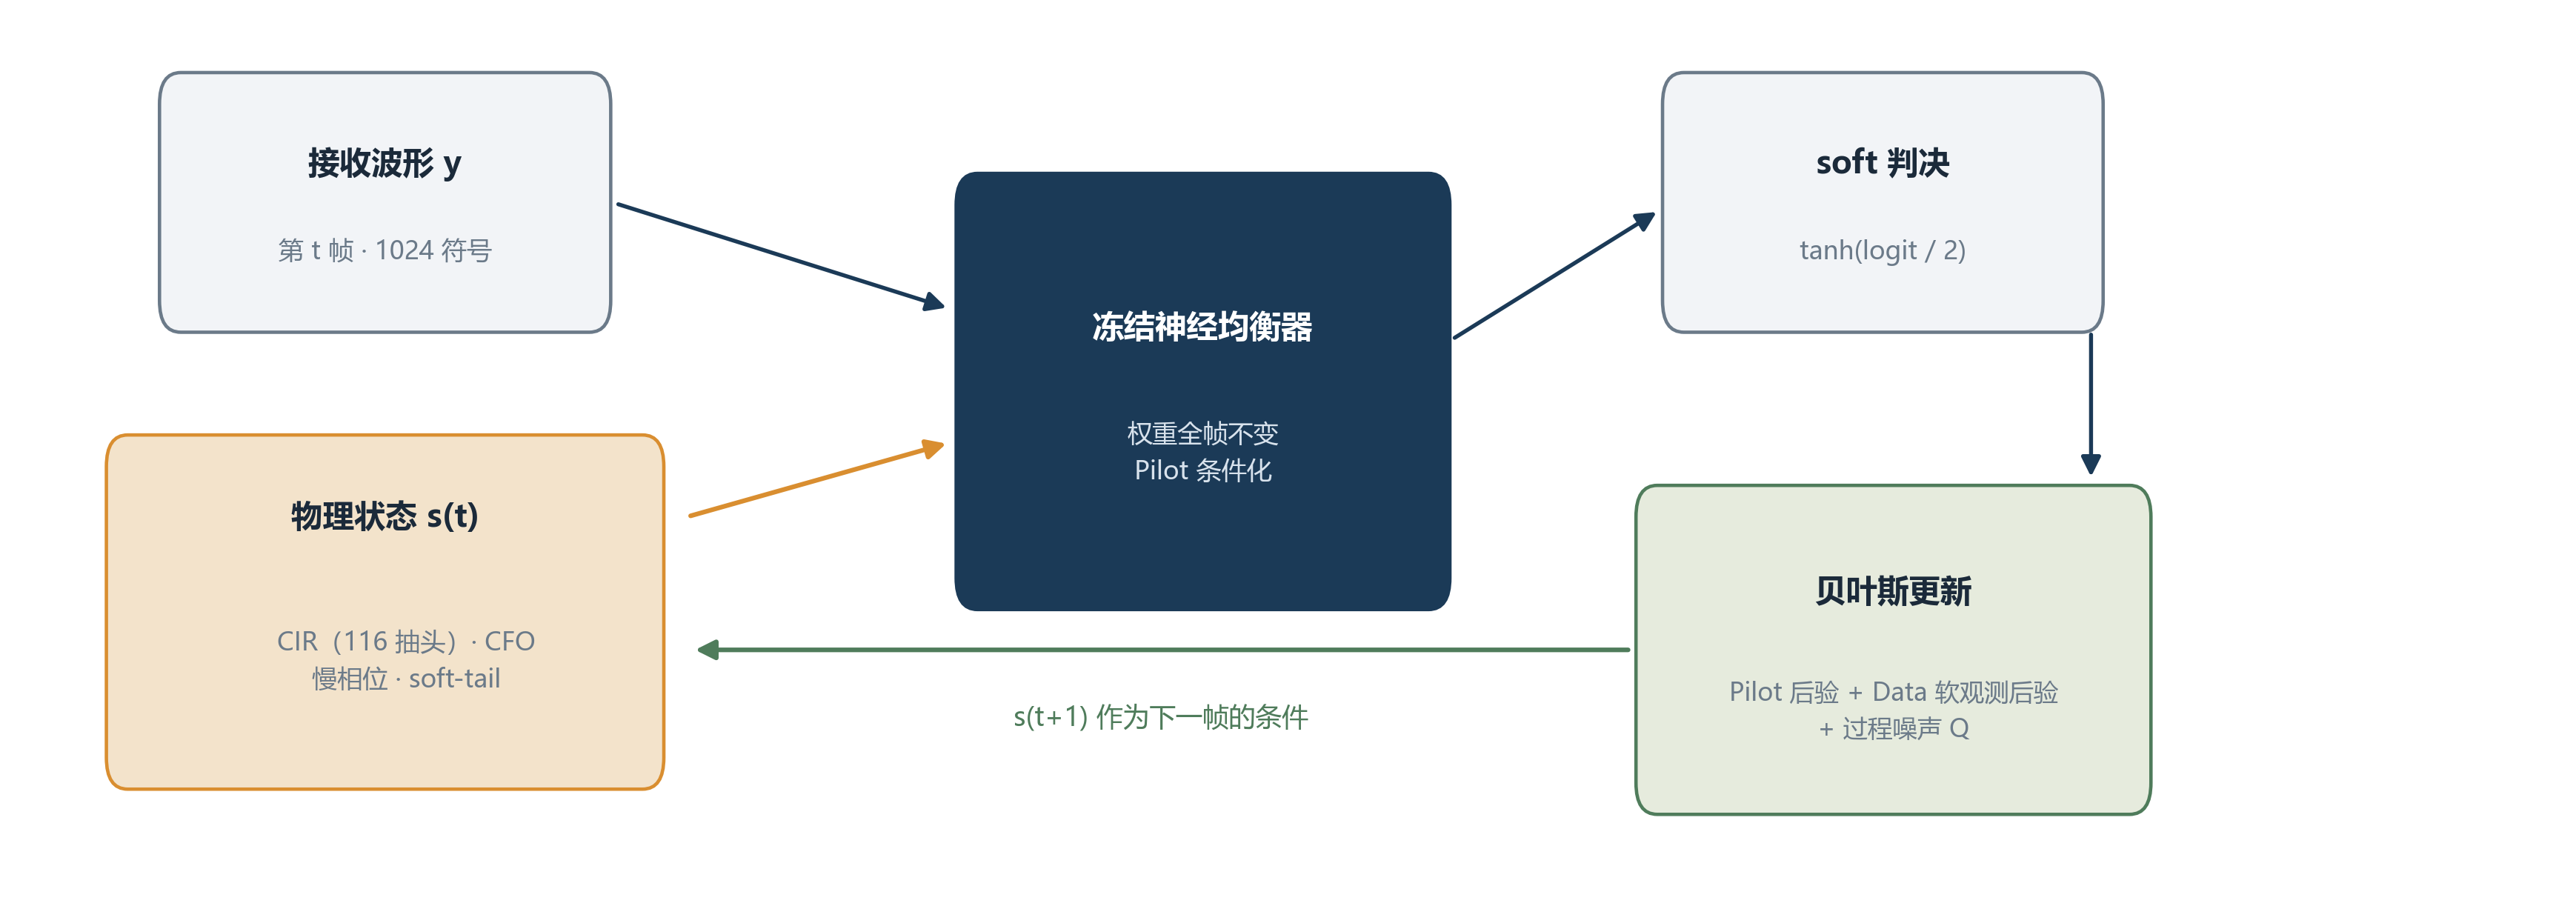
\includegraphics[width=0.95\linewidth]{figures/fig_online_loop.png}
\caption{在线闭环。冻结神经均衡器在物理状态 $s(t)$ 条件下输出软判决；贝叶斯更新利用 Adapt Pilot 与 Data 软观测递推 CIR 后验，所得 $s(t+1)$ 仅用于下一帧。}
\end{figure}

\subsection{贝叶斯递归 CIR 后验}

把 CIR 视为线性高斯状态，递推分四步。第一步，用 acquisition 帧的已知符号与 ridge $=10^{-2}$ 构造归一化先验均值 $\mathbf{m}_0$ 与协方差 $\boldsymbol{\Sigma}_0$。第二步，对每帧 Adapt Pilot 的已知符号做 Kalman 更新：

\begin{equation*}
\mathbf{K}_t=\boldsymbol{\Sigma}_t\boldsymbol{\phi}_t\left(\boldsymbol{\phi}_t^{\mathsf T}\boldsymbol{\Sigma}_t\boldsymbol{\phi}_t+\sigma^2\right)^{-1},
\end{equation*}

\begin{equation*}
\mathbf{m}_t\leftarrow\mathbf{m}_t+\mathbf{K}_t\left(y_t-\boldsymbol{\phi}_t^{\mathsf T}\mathbf{m}_t\right),\qquad
\boldsymbol{\Sigma}_t\leftarrow\left(\mathbf{I}-\mathbf{K}_t\boldsymbol{\phi}_t^{\mathsf T}\right)\boldsymbol{\Sigma}_t,
\end{equation*}

其中 $\boldsymbol{\phi}_t$ 由已知 Pilot 符号组成，$\sigma^2$ 为接收噪声方差。第三步，对 Data 位置使用模型软判决 $\hat{x}_t=\tanh(z_t/2)$ 作为伪观测，观测方程仍为 $y_t=\boldsymbol{\phi}_t^{\mathsf T}\mathbf{h}+n_t$，但行噪声改为

\begin{equation*}
R_t=\sigma^2+\sum_{l=0}^{L-1}|h_l|^2\operatorname{Var}(\hat{x}_{t-l}),\qquad
\operatorname{Var}(\hat{x})=1-\hat{x}^2.
\end{equation*}

当某个符号的软判决接近 0 时，其方差接近 1，该行在更新中被自动降权；当软判决接近 $\pm1$ 时，方差接近 0，该行接近已知符号。这样，低信噪比下的不可靠符号不会以硬判决的方式污染 CIR，也不需要按真实 SNR 调度。第四步，帧间对协方差加过程噪声 $\boldsymbol{\Sigma}\leftarrow\boldsymbol{\Sigma}+Q\mathbf{I}$，$Q=10^{-4}$，并把更新后的后验只用于下一帧，保持因果。

这一递推与经典 Kalman 滤波同构，区别在于 Data 行的观测是模型软判决而非真值，且行噪声依赖当前 CIR 与软符号方差。Kay 的估计理论给出了线性高斯状态下的最小均方误差更新形式\cite{kay1993}；本文把其用于 CIR 的跨帧递推，并把符号可靠性显式写入观测噪声。一个自然的替代是每帧对 Data 做最小二乘或 ridge 回归。但在 116 维状态、768 个 Data 符号且含错误符号的条件下，设计矩阵条件数很大，硬判决最小二乘会被错误符号主导；简单 Data LS 与 Pilot ridge 在开发诊断中正因欠定、相位残差与错误传播而失败。贝叶斯后验用先验协方差与行噪声正则化，等价于对 Data 行做加权 ridge，并把跨帧信息保留在协方差中。协方差的跨帧收缩解释了增长后饱和：随着帧数增加，后验方差下降，单帧 Data 观测对 CIR 的修正变小；当过程噪声 $Q$ 与信息增量平衡时，增益趋于稳态。0 dB 的后验还受错误传播影响，软符号方差只能部分抑制，不能完全消除。

\subsection{信息边界与归因}

在线可读的量为：已接收波形、Adapt Pilot 已知符号、模型 soft 输出 $\tanh(z/2)$、以及由 Pilot 驱动的 CIR/CFO/相位/tail 估计。在线禁止读取：Data 发送符号或比特、仿真真实 CIR/相位/CFO、Reward Pilot 回流内循环、未来帧标签。Data 段的波形参与均衡与无标签判决反馈，但 Data 标签不进入任何在线更新、选择、验收或阈值设定；Data 后验使用的是模型软判决作为伪观测，不是真值。Reward Pilot 只在动作后用于验收，本文的 CIR 递推不读取它。真实 CIR 只用于事后 NMSE/oracle 诊断，Data 标签只用于事后 BER。

归因上，Frozen 与 Bayes 共享 checkpoint、acquisition 先验、tail 规则、Pilot 预算与波形，唯一差异是 CIR 后验。因此本文报告的增益是物理状态增益，不是网络权重更新带来的增益。本文的全部在线适配都作用于 CIR 后验；网络权重在部署阶段保持冻结。从信息使用角度看，Frozen 只使用 acquisition 帧构造一次 CIR；Bayes 使用每帧 Adapt Pilot 与 Data 波形，但把这些观测压缩到 116 维状态后验中，而不是写入网络权重。两臂接收到的波形相同，差别在于是否让跨帧观测改变状态估计。

\subsection{复杂度与因果性}

每帧的贝叶斯更新只涉及 116 维状态与 1024 个观测行，Pilot 后验与 Data 后验合计约 30 ms（当前 GPU 的 profile：Pilot 8.6–10.4 ms，Data 19.3–21.7 ms）。主要成本仍在冻结网络前向：单次前向约 400 ms；tail 若独立前向再加约 400 ms，总耗时约 830 ms；tail 复用与独立前向逐位一致，可把总耗时降到约 435 ms，约为 102.4 ms 帧预算的 4.2 倍。因此当前实现不满足实时性，模型前向是瓶颈。本文把逐帧延迟与显存列为待补的工程项，而不是已完成的指标。因果性方面，第 $t$ 帧的判决只使用第 $t$ 帧及之前的观测与第 $t-1$ 帧结束时的 CIR 后验；更新后的 CIR 不用于重新解码本帧。这个时序约束使 Bayes 与 Frozen 的差异不来自“看了答案再改”，也使确认结果可以与在线部署的因果流程对应。
